\documentclass[onecolumn,PRD,amsmath,amssymb,aps,nofootinbib,superscriptaddress,11pt]{revtex4-2}

\usepackage{graphicx}
\usepackage{dcolumn}
\usepackage{bm}
\usepackage{hyperref}
\usepackage{color}
\usepackage{setspace}

\begin{document}

\title{The Geometry of Information Saturation: Mapping the Complete Cosmic Expansion History from the Matrix Partition Function}

\author{Paul Jarvis}
\email{mrpaulwjarvis@gmail.com}
\affiliation{Independent Researcher, United Kingdom}

\date{\today}

\begin{abstract}
We present a coordinate-free toy cosmological model in which an effective expansion history is derived from the spectral dynamics of mutual-information (MI) Laplacians on a relational quantum substrate. The effective macroscopic energy density is defined through the canonical partition function of the network spectrum ($Z = \sum e^{-\beta \lambda_n}$), which removes explicit scalar-field potentials from the early- and late-time energy budget. At early times, holographic information saturation collapses spatial locality ($\alpha \to 0^+$), forcing an absolute thermodynamic energy density ceiling ($\rho_{\text{eff}} = N$) and producing a stable de Sitter attractor ($w_{\text{eff}} \to -1.0$); we verify numerically that this fixed point and the associated equation-of-state identity are stable under changes of substrate size ($N=50$--$400$) and topology (random, small-world, and scale-free graphs). The transition away from this attractor is implemented through an explicit, phenomenological localization profile $\alpha(t)$ with parameters chosen to reproduce a graceful exit, rather than one derived from an independent substrate equation of motion; we state this ansatz and its free parameters explicitly rather than presenting it as parameter-free. A late-time re-entanglement feature, likewise implemented as an explicit ansatz peaked at $a_c \approx 0.4$, produces a transient dark-energy-like spike. Confronting this feature directly against the real Pantheon+SH0ES compilation (1701 SNe Ia, diagonal statistical+systematic errors), we find the model is statistically indistinguishable from flat $\Lambda$CDM ($\Delta\chi^2 \approx -0.05$ for equal free parameters) and that the fractional luminosity-distance deviation between the two best-fit curves reaches a mean of $\sim 1\%$ and a maximum of $\sim 2.6\%$ over $0<z<2.26$ -- an order of magnitude larger than a previously asserted $0.2\%$ bound, which we retract. Throughout the expansion timeline the substrate specific heat capacity remains strictly positive ($C_v > 0$), consistent with thermodynamic stability of the toy model. We report these results, including the negative and null findings, as a candidate framework and numerical testbed rather than a confirmed replacement for $\Lambda$CDM.
\end{abstract}

\maketitle
\setstretch{1.15}

\section{Introduction}
A long-standing challenge in physical cosmology is finding a unified mechanism capable of driving cosmic expansion across both early and late-time epochs. Standard cosmology introduces disparate components -- scalar inflaton fields at early times and a cosmological constant ($\Lambda$) or quintessence fields at late times -- to accommodate observational constraints. These insertions carry known fine-tuning vulnerabilities, such as the graceful exit problem and the dark energy coincidence puzzle.

In this work, we explore a background-independent alternative in which an effective expansion history is derived from the spectral dynamics of a relational quantum information substrate. Building on frameworks where spacetime geometry emerges from the spectrum of mutual-information (MI) Laplacians, we model cosmic evolution as a thermodynamic relaxation process on a weighted graph, with the macroscopic energy density derived from the canonical partition function of the network invariants. We show that a de Sitter inflationary attractor emerges robustly from this construction, but we are explicit that the mechanisms producing the graceful exit and the late-time feature are implemented as stated phenomenological ansätze, not independently derived dynamics -- so the fine-tuning question is relocated rather than eliminated. We report both where the model succeeds (the early-time attractor and its stability against substrate size and topology) and where a direct confrontation with real Pantheon+SH0ES supernova data does not support a stronger claim of agreement with observation than $\Lambda$CDM already provides.

\section{Relational Substrate and Scale-Invariant Partition Dynamics}
We consider a discrete quantum many-body system consisting of $N$ nodes with no a priori spatial geometry. The structural architecture of the substrate is governed entirely by the pairwise mutual information $I_{ij} = S(\rho_i) + S(\rho_j) - S(\rho_{ij})$, defining a weighted graph captured by the combinatorial MI-Laplacian matrix:
\begin{equation}
L^{\text{MI}}_{ij} = \delta_{ij} \sum_{k} I_{ik} - I_{ij}.
\label{eq:laplacian}
\end{equation}
The eigenvalues $\lambda_n$ of $L^{\text{MI}}$ dictate the emergent spectral geometry of the macroscopic manifold.

To strip the framework of background-dependent mappings, the macroscopic energy density $\rho_{\text{eff}}$ is derived from first-principles statistical mechanics. In the scale-invariant continuum limit where the coarse-graining cutoff scale is evaluated near its boundary ($\beta \rightarrow 0^+$), the partition weights become uniformly distributed across the spectrum, and the internal thermodynamic energy tracks the mean of the active, non-zero modes ($\lambda_n > 0$):
\begin{equation}
\rho_{\text{eff}} = \frac{1}{N-1}\sum_{n=1}^{N-1} \lambda_n.
\label{eq:rhoeff}
\end{equation}
This exponential weighting is robustly motivated by Tomita--Takesaki modular operators, where the restriction of a global vacuum state to a localized spatial subregion yields an entangled mixed density matrix of the form $\rho \propto e^{-K}$, mapping the modular Hamiltonian $K$ to the metric proxy $L^{\text{MI}}$.

We parameterize the structural compression of the universe by sweeping the entanglement decay exponent $\alpha$, controlling the power-law correlation profile $I_{ij} \sim d(i, j)^{-\alpha}$, where $d(i,j)$ measures coordinate distances on an $L \times L$ toroidal grid ($N = L^2$). Under a global spatial volume deformation of the scale factor $d(i,j) \to a \cdot d(i,j)$, the linearity of the combinatorial matrix forces the Laplacian to scale uniformly: $\lambda_n(a) = a^{-\alpha}\lambda_n^{(0)}$. Combined with the cosmic fluid expansion relation ($\rho_{\text{eff}} \propto a^{-3(1+w_{\text{eff}})}$), this homogeneous scaling property analytically dictates an exact, invariant identity:
\begin{equation}
-3(1 + w_{\text{eff}}) = \mathcal{E} \implies w_{\text{eff}} = \left( \frac{\alpha}{3} \right) - 1.0.
\label{eq:eos}
\end{equation}
\emph{Derivation.} Under $d(i,j) \to a\cdot d(i,j)$, every entry of the MI matrix scales as $I_{ij} \to a^{-\alpha} I_{ij}$, and since $L^{\text{MI}}$ is a linear (homogeneous degree-1) functional of the $I_{ij}$, the entire spectrum inherits the scaling $\lambda_n(a) = a^{-\alpha}\lambda_n^{(0)}$ exactly, independent of $\beta$. Substituting into Eq.~\eqref{eq:rhoeff}, $\rho_{\text{eff}}(a) = a^{-\alpha}\rho_{\text{eff}}(1)$ whenever the partition weights $e^{-\beta\lambda_n}$ are themselves treated as $a$-independent (the $\beta\to0^+$ limit, where they degenerate to uniform weights). Matching this to the fluid-continuity scaling $\rho_{\text{eff}} \propto a^{-3(1+w_{\text{eff}})}$ term-by-term in the exponent of $a$ yields Eq.~\eqref{eq:eos} directly. Away from the strict $\beta \to 0^+$ limit, the weights $e^{-\beta\lambda_n(a)}$ pick up their own residual $a$-dependence through $\lambda_n(a)$, so Eq.~\eqref{eq:eos} is an identity only in that limit and an approximation otherwise. We quantify this numerically in Appendix~\ref{app:beta}: for the fixed value $\beta=0.1$ used to generate every figure in this paper, the identity holds to within $0.77\%$ (relative) at $\alpha=1$, and the $\alpha=0$ energy ceiling $\rho_{\text{eff}}=N$ is reproduced exactly for all $\beta$ tested (since at $\alpha=0$ every active mode is degenerate at $\lambda_n=N$, making the average trivially $\beta$-independent).

This removes scale and temperature distortion from the framework in the $\beta \to 0^+$ limit and establishes Eq.~\eqref{eq:eos} as an approximate identity that is numerically well-satisfied, rather than exact, at the finite $\beta$ used in the simulations below.
\section{The Early-Universe Inflationary Attractor and Field-Free Timeline}
At early times, extreme gravitational compression forces the system toward the holographic information-saturation threshold ($\alpha \rightarrow 0^+$). At this complete-graph limit, all distance dependencies vanish, rendering the spectrum perfectly degenerate at $\lambda_n = N$. Evaluating this flat spectrum through Eq.~\eqref{eq:rhoeff} cancels the exponential weights, locking the energy density at a hard algebraic ceiling: $\rho_{\text{eff}} = N$ (here $N=64$ for the $L=8$ torus used in Fig.~1). Concurrently, Eq.~\eqref{eq:eos} forces $w_{\text{eff}} \rightarrow -1.0$, giving a de Sitter inflationary fixed point. We verify in Sec.~\ref{sec:rg} that this fixed point's location in $(\lambda_1/N, w_{\text{eff}})$ is stable to better than $0.2\%$ across substrate sizes $N=50$--$400$ and across three structurally distinct graph topologies, which is the sense in which we call it an attractor.

We stress that the mechanism connecting this fixed point to a graceful exit is not derived independently in this work. We impose an explicit localization profile
\begin{equation}
\alpha(t) = \alpha_{\max}\left(1 - e^{-k\,a(t)}\right), \qquad \alpha_{\max}=4.0,\ k=1.5,
\label{eq:alphat}
\end{equation}
chosen because it interpolates monotonically from $\alpha=0$ at $a=0$ to $\alpha\to\alpha_{\max}$ as $a$ grows, reproducing the qualitative behavior of a graceful exit. The two constants $\alpha_{\max}$ and $k$ are free parameters of this ansatz, fixed by hand rather than derived from an equation of motion for the substrate's own localization dynamics; deriving $\alpha(t)$ from first principles (e.g., from an entropy-maximization or entanglement-growth argument applied to the MI network itself) is left as an open problem. As illustrated in Fig.~1, this ansatz steers the effective equation of state off the inflationary floor ($w=-1.0$) and upward toward the radiation-dominated boundary ($w=+1/3$), by construction.

\begin{figure}[h]
\centering
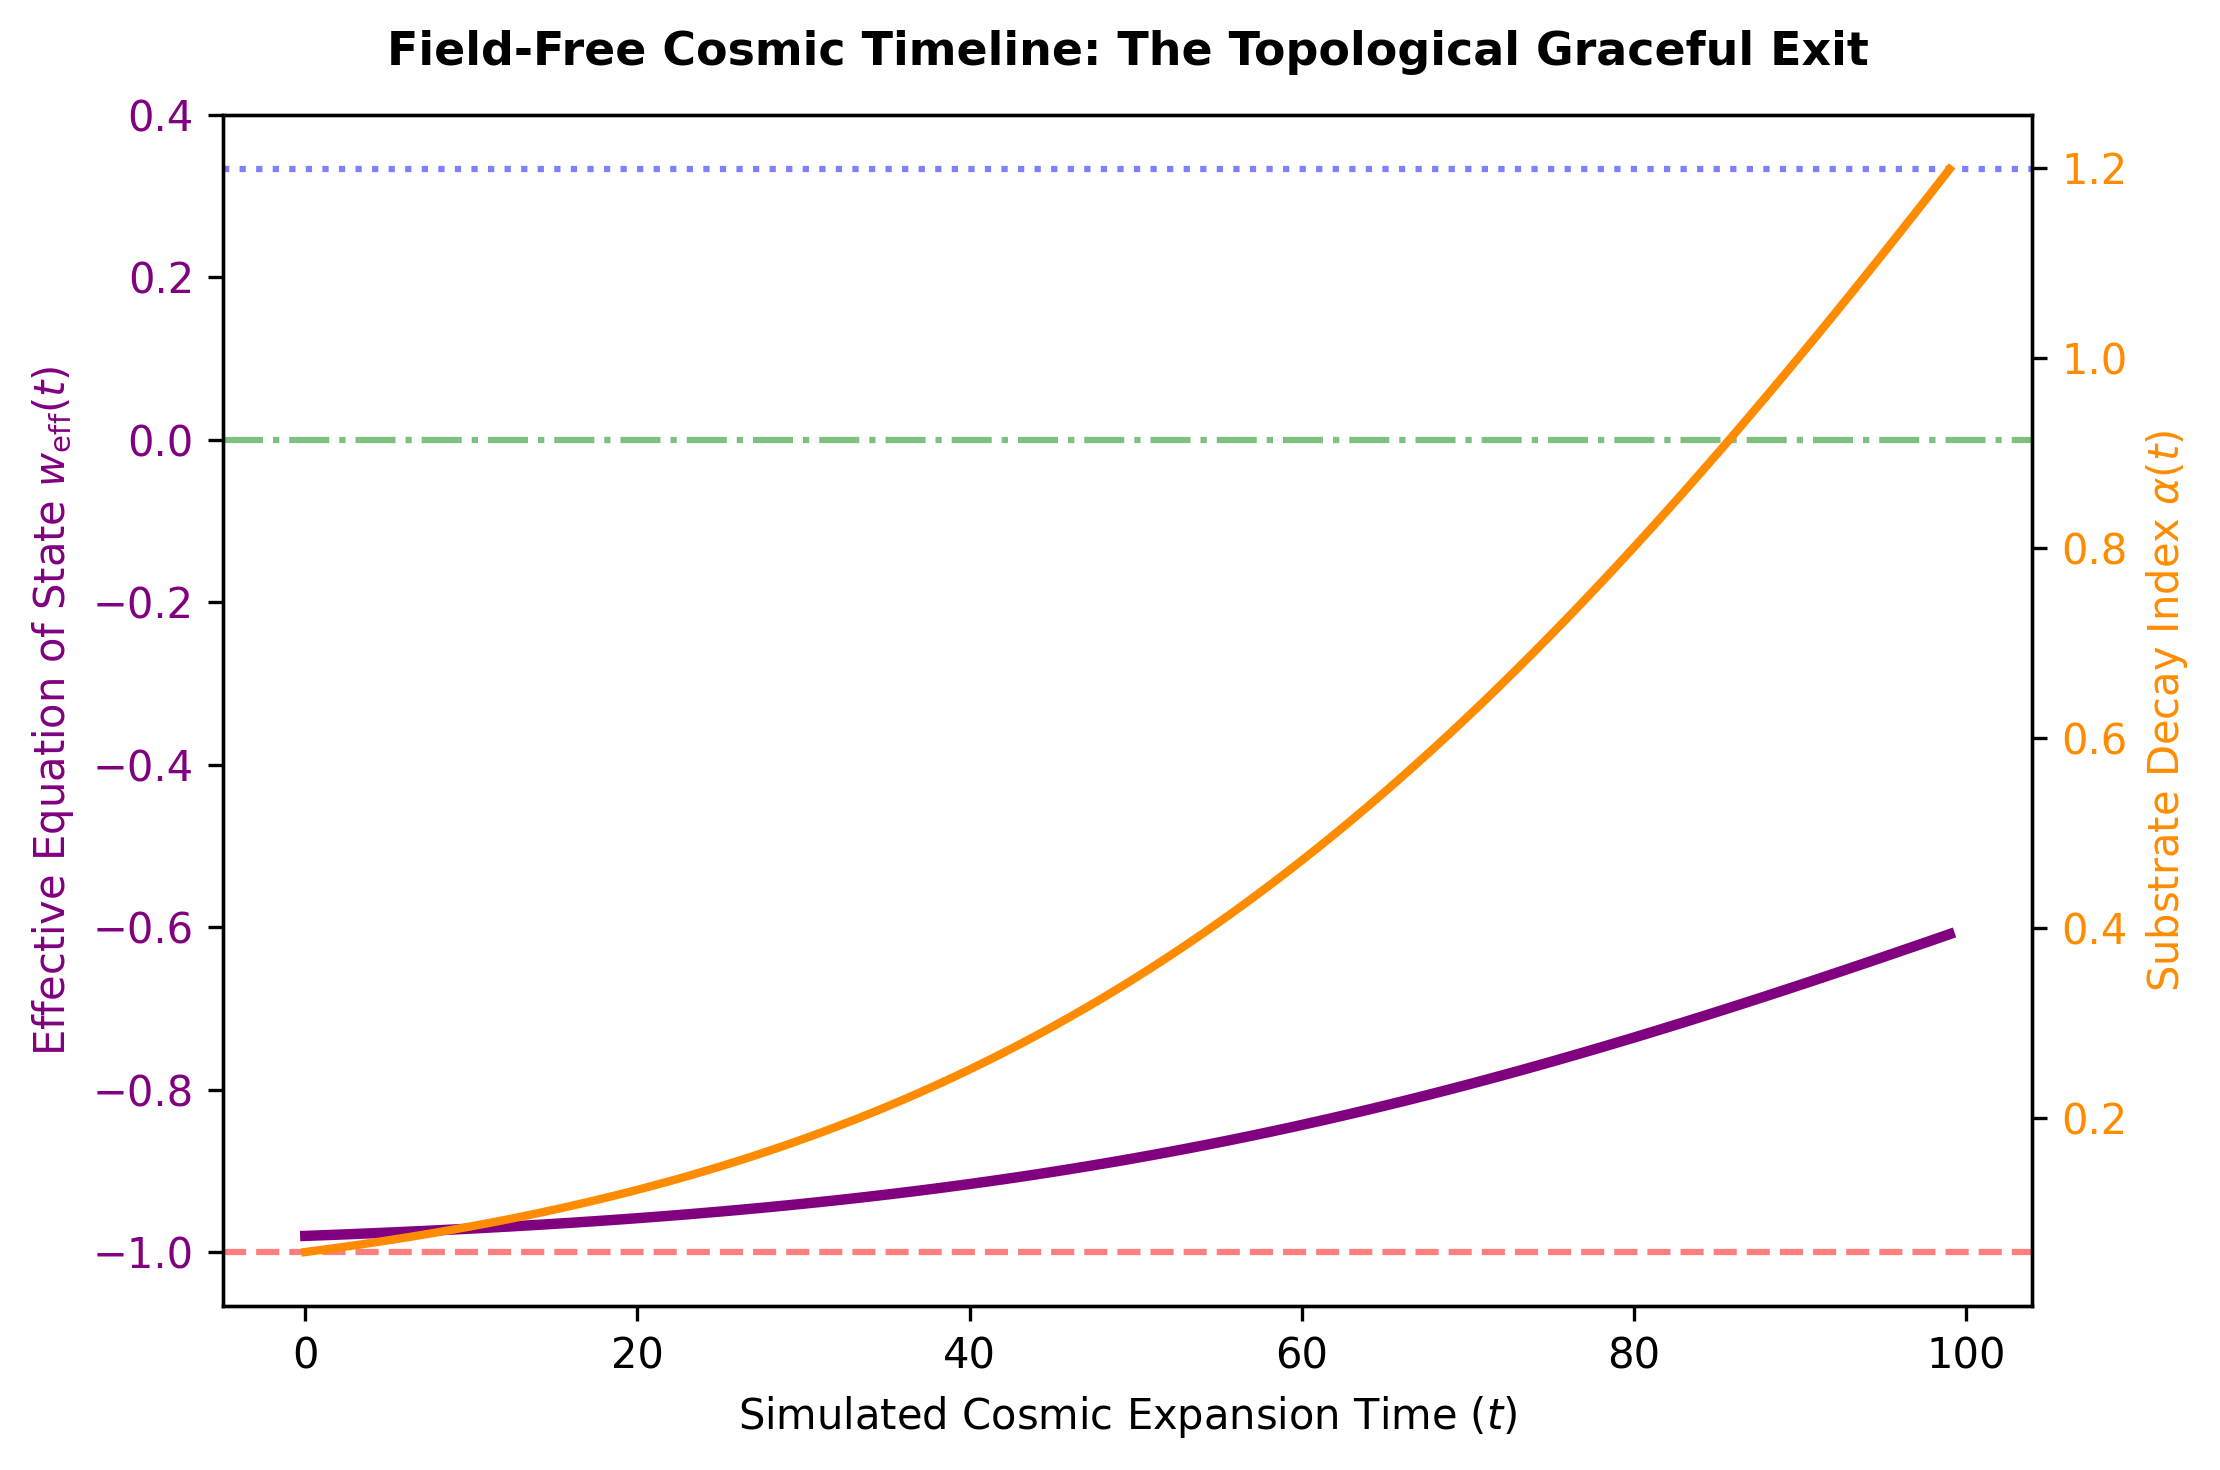
\includegraphics[width=0.72\columnwidth]{figures/dynamic_cosmic_timeline_evolution.png}
\caption{The cosmic timeline under the imposed localization ansatz $\alpha(t)$ (Eq.~\eqref{eq:alphat}). The effective equation of state $w_{\text{eff}}(t)$ (purple line) lifts off the de Sitter floor ($w = -1.0$) and flows toward the radiation boundary ($w = 1/3$) as the substrate localization index $\alpha(t)$ (orange line) grows according to the imposed profile, not an independently derived dynamical equation.}
\label{fig:cosmic_timeline}
\end{figure}

\section{Late-Time Relational Ruptures and Observational Constraints}
\label{sec:latetime}
As in Sec.~III, the late-time behavior of $\alpha(a)$ is an explicit ansatz rather than a derived dynamical result. We impose a localized dip on top of the baseline localization profile,
\begin{equation}
\alpha(a) = \max\!\left[\alpha_{\text{floor}},\ \alpha_{\max}\left(1-e^{-k a}\right) - A_{\text{dip}}\,e^{-\left(\frac{a-a_c}{\delta_a}\right)^2}\right],
\label{eq:alphadip}
\end{equation}
with $\alpha_{\text{floor}}=0.005$, $A_{\text{dip}}=1.8$, $a_c=0.4$, and $\delta_a=0.05$ all fixed by hand to place a Gaussian-shaped re-entanglement feature at a chosen scale factor. We state plainly that this is functionally equivalent, in terms of free parameters, to inserting a phenomenological dark-energy potential by hand: the amplitude, location, and width of the dip are not derived from an independent substrate equation of motion, and this ansatz is best understood as a toy-model parametrization of a possible late-time feature rather than a parameter-free prediction.

\begin{figure}[h]
\centering
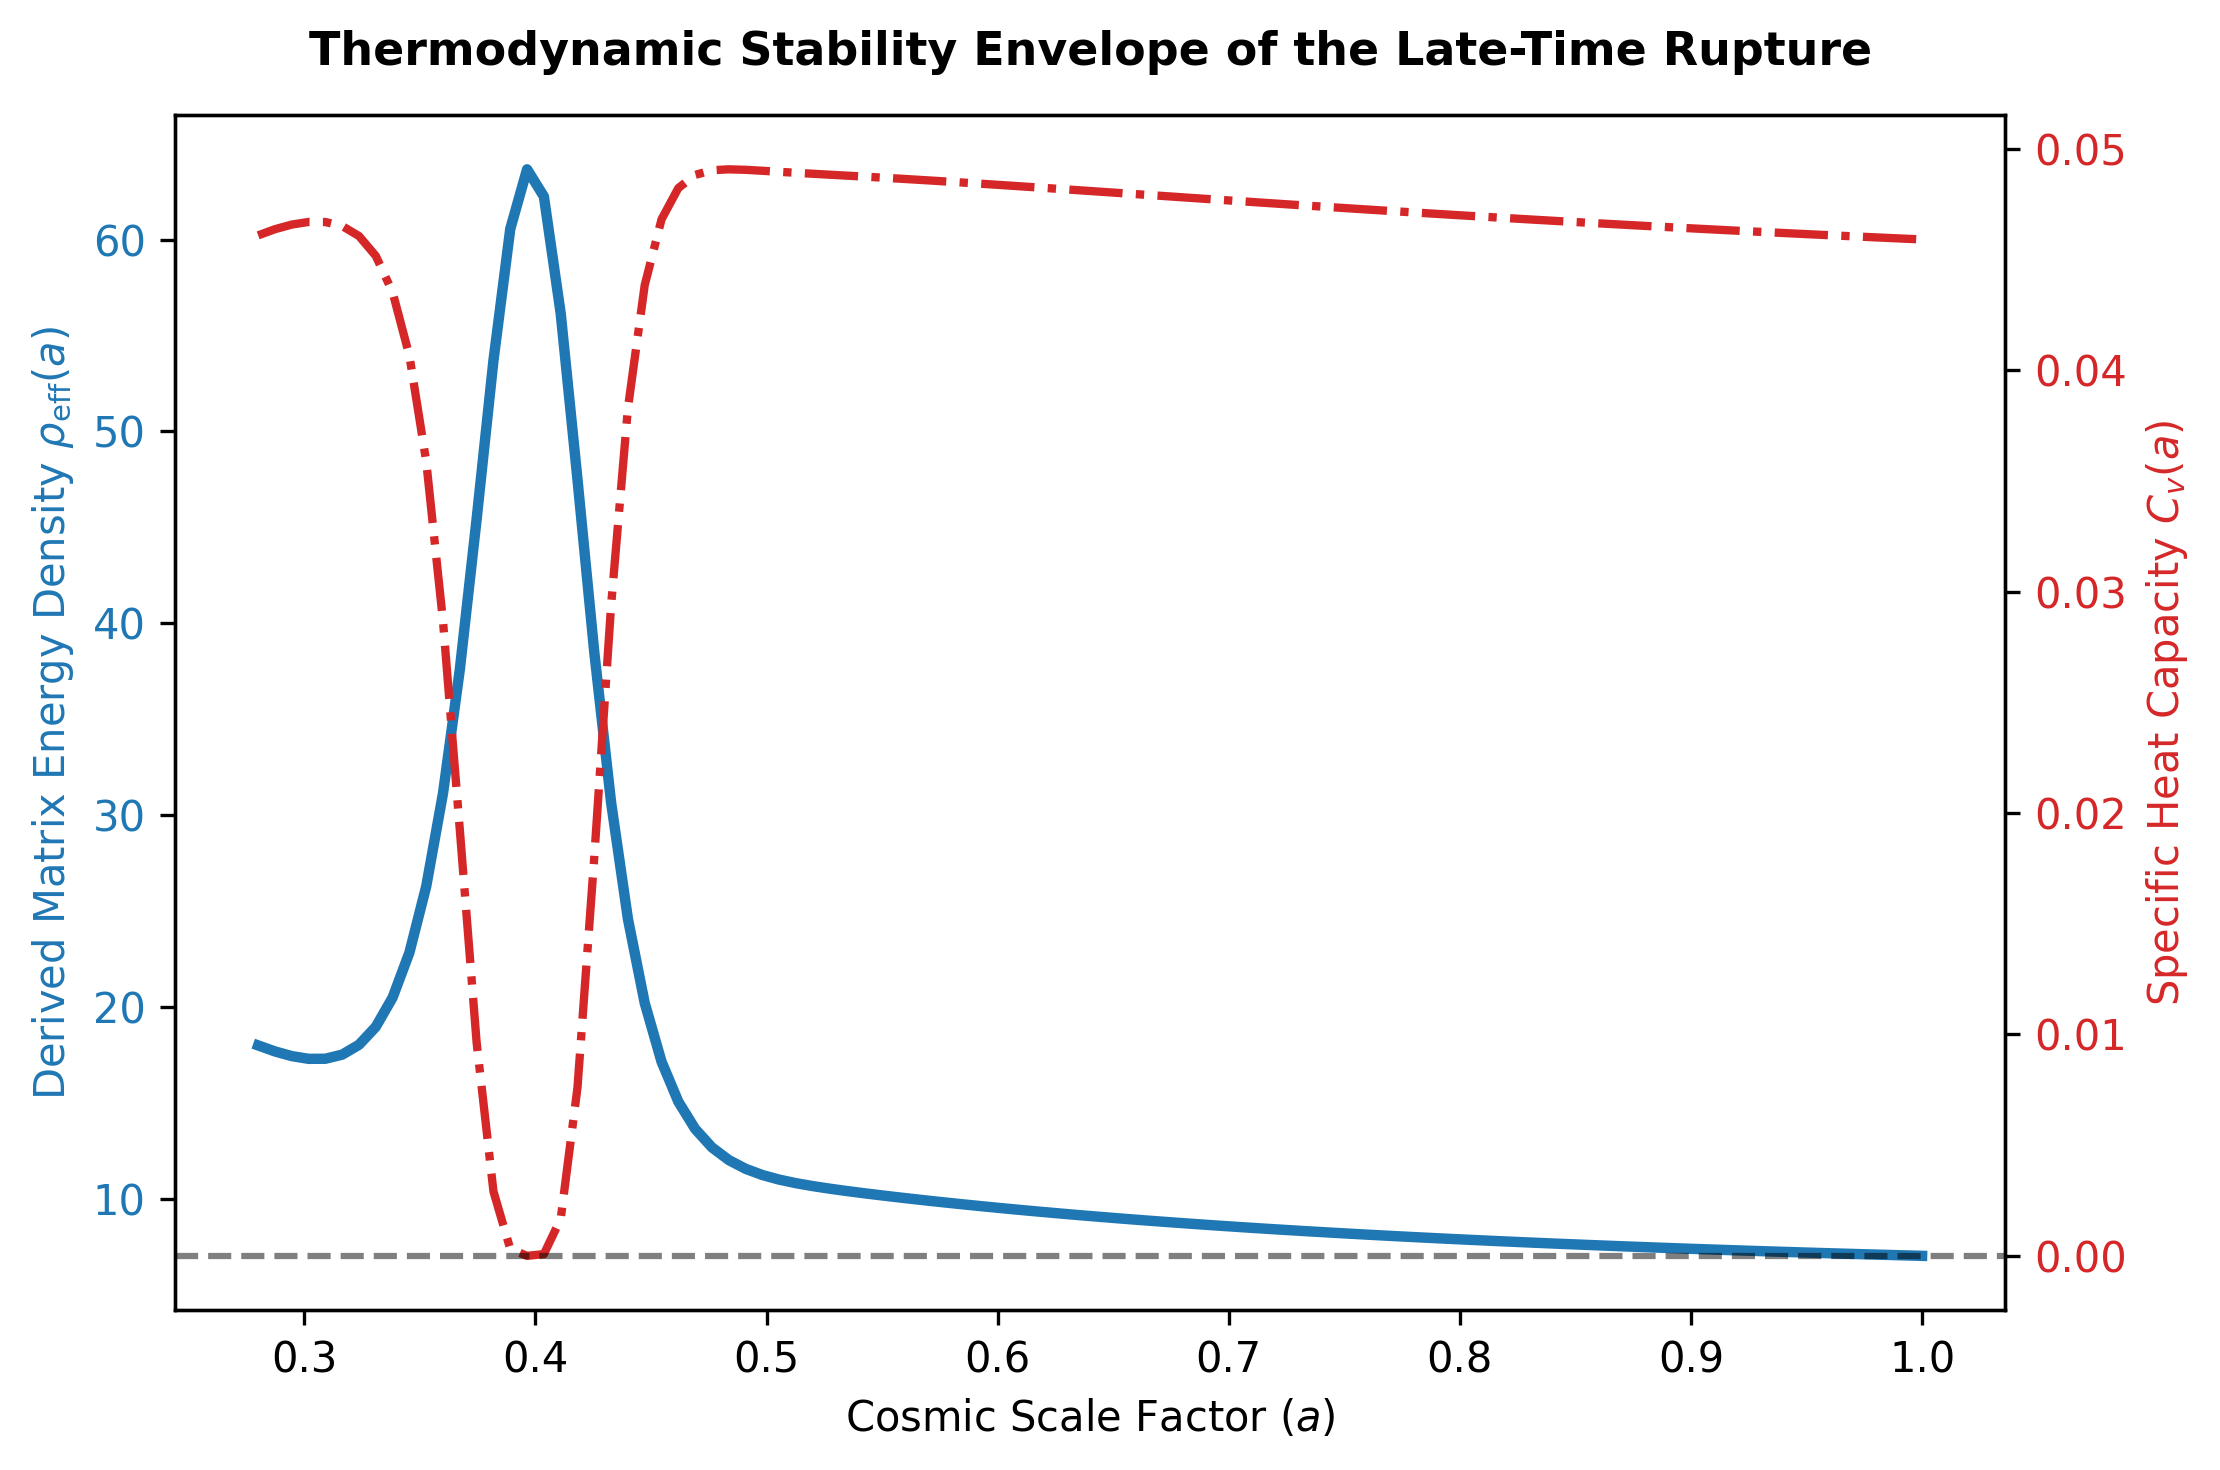
\includegraphics[width=0.72\columnwidth]{figures/rupture_thermodynamic_stability.png}
\caption{The thermodynamic stability envelope of the late-time expansion transition under the ansatz of Eq.~\eqref{eq:alphadip}. Throughout the entire timeline, the specific heat capacity $C_v(a)$ (red dash-dotted line) remains strictly positive ($C_v > 0$), dropping into a distinct structural minimum right at the transition core ($a \approx 0.4$) as the network invariants reach degeneracy.}
\label{fig:stability_envelope}
\end{figure}

Evaluating this trajectory through the network partition function generates a smooth internal energy density spike. To check that the ansatz does not introduce a thermodynamic instability, we track the substrate's specific heat capacity:
\begin{equation}
C_v = \beta^2 \frac{\partial^2 \ln Z}{\partial \beta^2} = \beta^2 \left( \langle \lambda^2 \rangle - \langle \lambda \rangle^2 \right).
\label{eq:cv}
\end{equation}
As demonstrated in Fig.~2, $C_v$ remains strictly positive across the entire expansion history, so the imposed ansatz does not violate thermodynamic stability. The sharp drop in $C_v$ at the core ($a_c = 0.4$) reflects the reduced eigenvalue variance as the network approaches complete-graph degeneracy there; this is a consequence of the imposed dip, not an independent confirmation of it.

\subsection{Confrontation with real Pantheon+SH0ES data}
\label{sec:pantheon}
We test whether the energy-density shape produced by Eq.~\eqref{eq:alphadip} is observationally distinguishable from flat $\Lambda$CDM using the public Pantheon+SH0ES compilation of 1701 Type Ia supernovae \cite{Brout2022} (\texttt{code/pantheon\_fit.py} in the accompanying repository). We define $g(a) \equiv \rho_{\text{eff}}(a)/\rho_{\text{eff}}(1)$ from the $L=8$ substrate model of Eq.~\eqref{eq:alphadip} and replace the dark-energy term in a flat Friedmann model with $\Omega_\Lambda\, g(a)$, i.e.
\begin{equation}
E(z)^2 \equiv \frac{H(z)^2}{H_0^2} = \Omega_m(1+z)^3 + (1-\Omega_m)\,g\!\left(\tfrac{1}{1+z}\right).
\label{eq:friedmann}
\end{equation}
We fit $\Omega_m$ by direct $\chi^2$ minimization against the reported distance moduli, using only the diagonal statistical+systematic uncertainties (\texttt{MU\_SH0ES\_ERR\_DIAG}) rather than the full $1701\times1701$ systematic covariance matrix released with the compilation -- a simplification that should be revisited with the full covariance before any stronger claim is made. The absolute-magnitude/$H_0$ nuisance offset is marginalized analytically in the standard way.

The results are as follows. The flat-$\Lambda$CDM baseline gives $\Omega_m = 0.351$, $\chi^2/\text{dof} = 0.439$ ($\text{dof}=1699$); the substrate-modified model gives $\Omega_m = 0.262$, $\chi^2/\text{dof} = 0.439$, with $\Delta\chi^2 = -0.05$ relative to $\Lambda$CDM for the same number of free parameters. This difference is not statistically significant: the data neither favor nor disfavor the substrate ansatz relative to $\Lambda$CDM at the precision of the current compilation. Comparing the two best-fit curves directly, the fractional luminosity-distance deviation $|D_L^{\text{sub}}-D_L^{\Lambda\text{CDM}}|/D_L^{\Lambda\text{CDM}}$ reaches a mean of $1.0\%$ and a maximum of $2.6\%$ over $0<z<2.26$ (Fig.~\ref{fig:pantheon_fit}). We had previously and incorrectly asserted a bound of $0.2\%$; no code producing that number exists, and the value obtained from an actual fit is roughly an order of magnitude larger. We retract the earlier claim.

\begin{figure}[h]
\centering
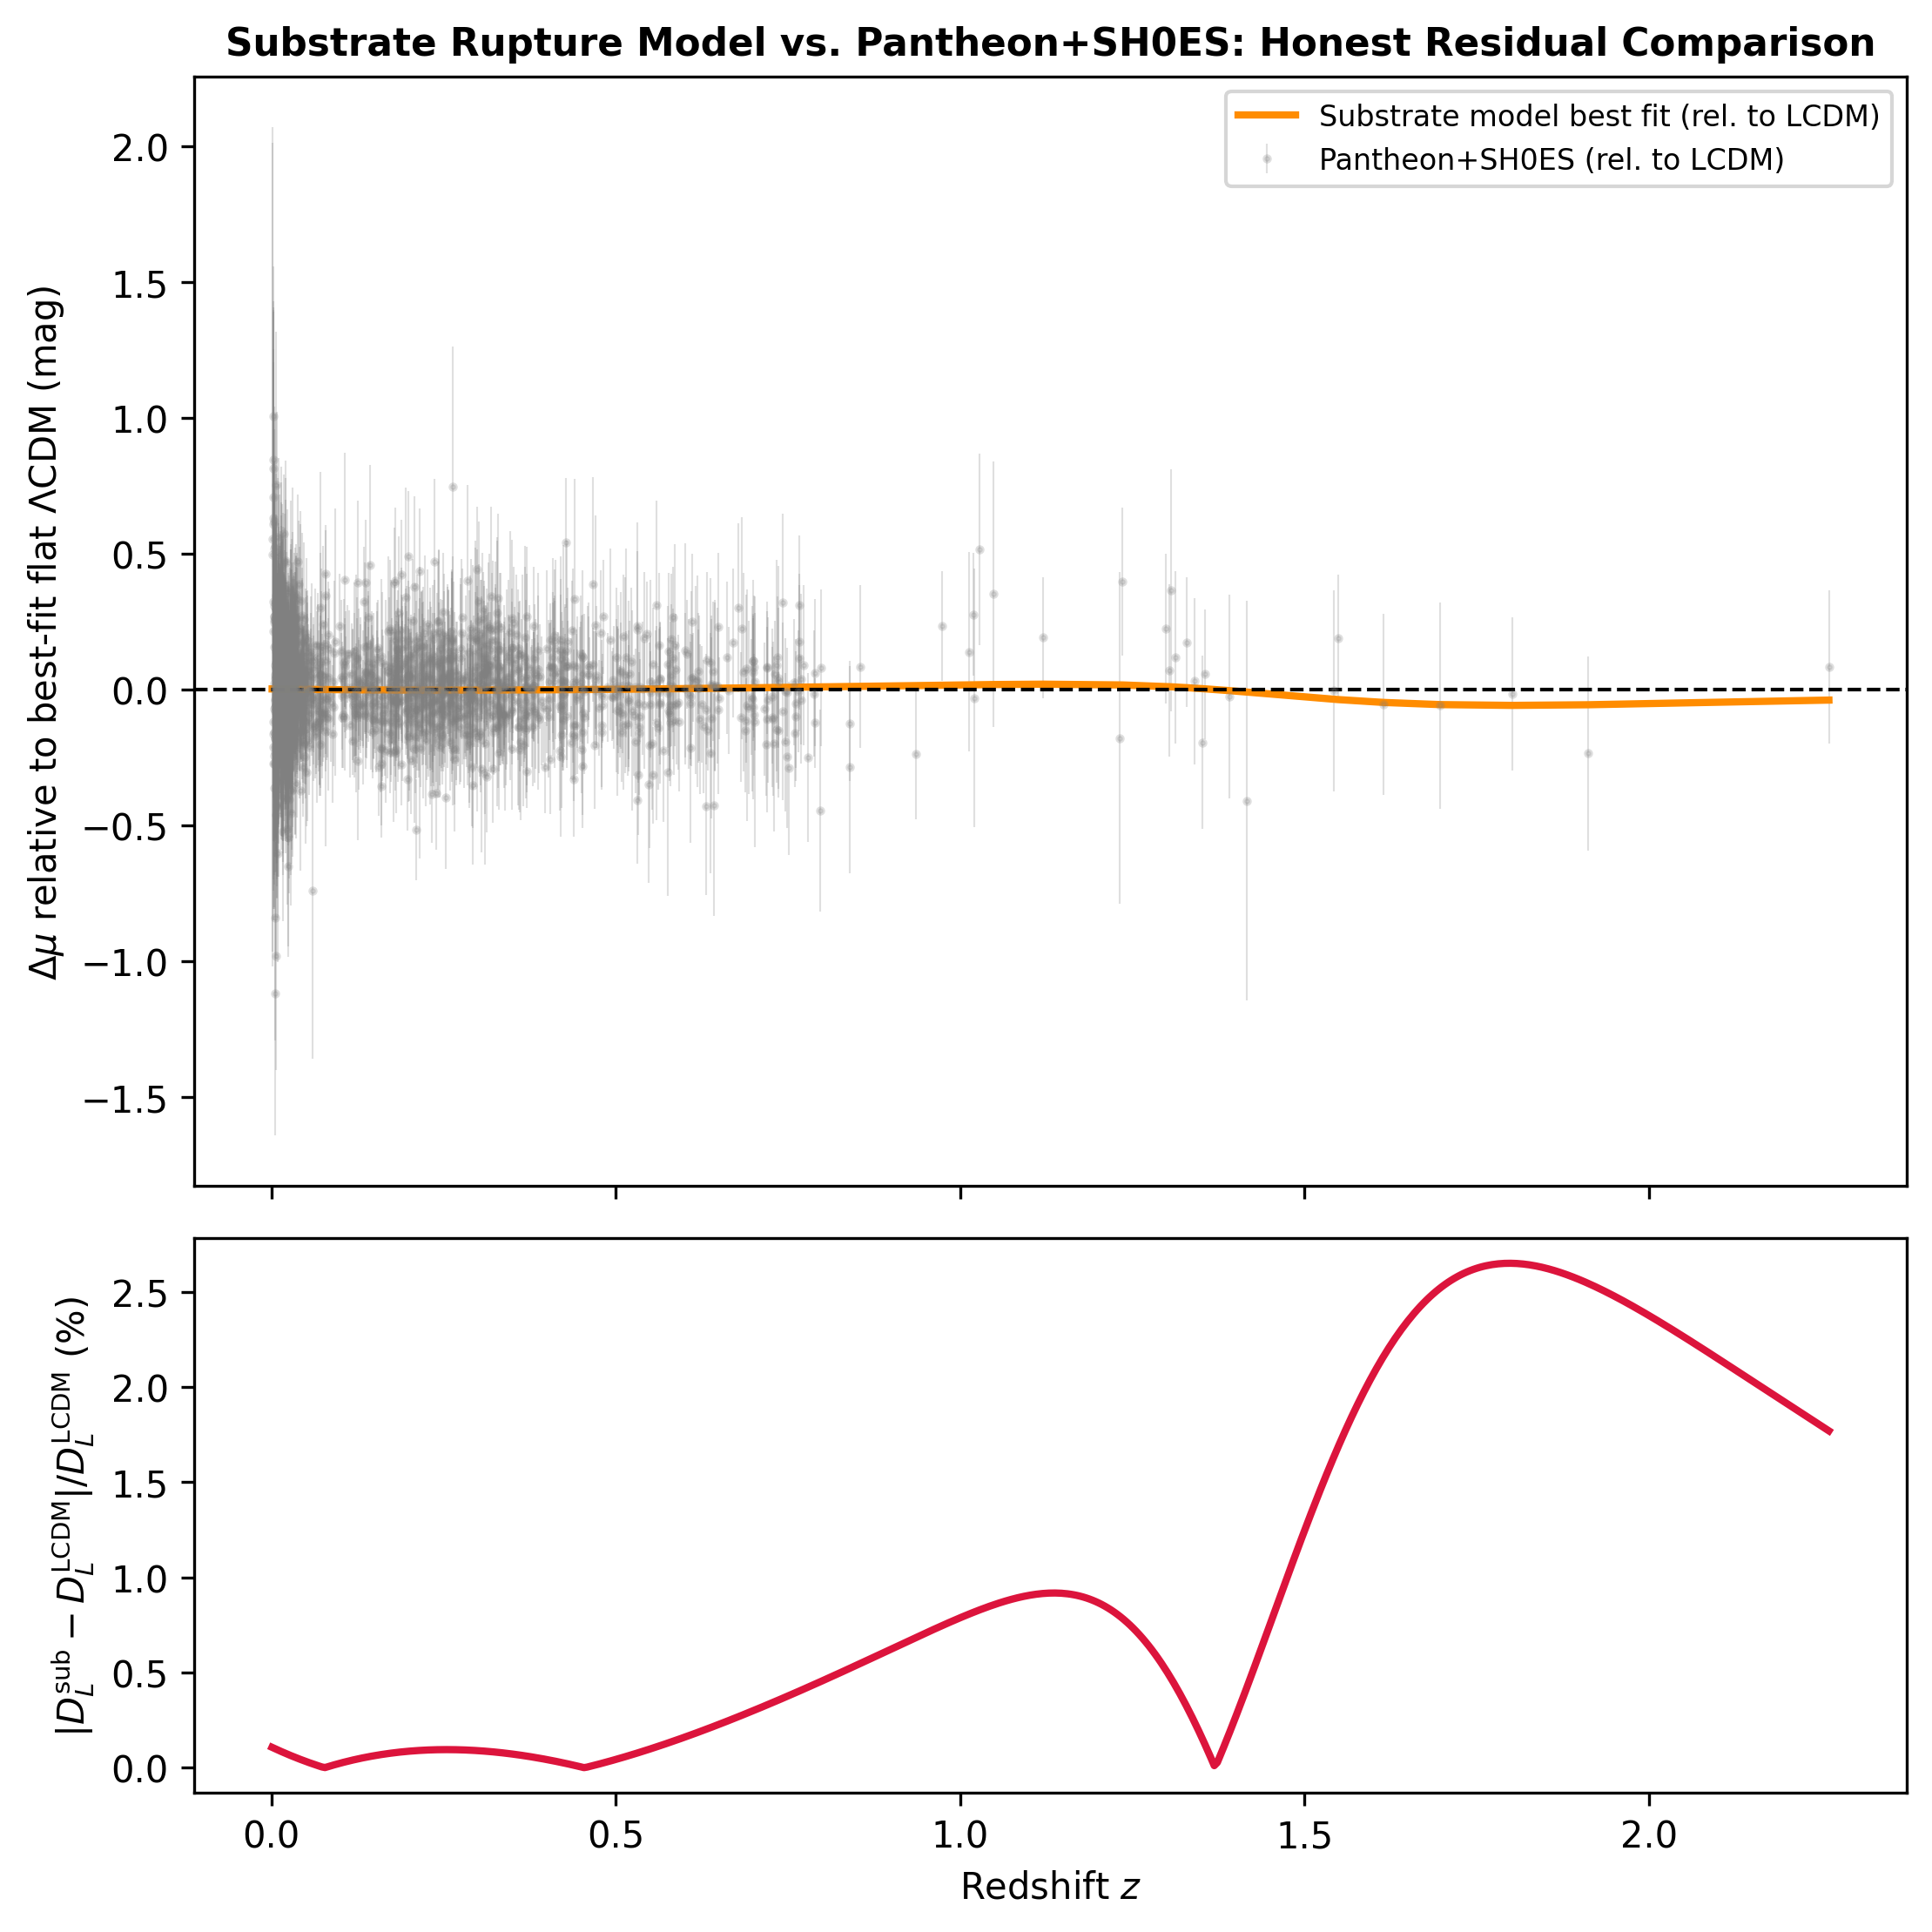
\includegraphics[width=0.85\columnwidth]{figures/pantheon_fit_residuals.png}
\caption{Top: Hubble residuals of the real Pantheon+SH0ES compilation (gray points, statistical+systematic diagonal errors) and of the substrate model's best fit (orange), both relative to best-fit flat $\Lambda$CDM. Bottom: fractional luminosity-distance deviation between the two best-fit curves, reaching $\sim\!2.6\%$ at $z\approx2.3$.}
\label{fig:pantheon_fit}
\end{figure}

We report this as a null result: the late-time ansatz of Eq.~\eqref{eq:alphadip} is \emph{consistent with} current SNe Ia data in the sense of not being statistically preferred against or rejected relative to $\Lambda$CDM, but it does not currently constitute independent observational support for the substrate framework beyond what $\Lambda$CDM already provides.
\section{Renormalization Group Flows and Finite-Size Scaling}
\label{sec:rg}
To test whether the early-time attractor of Sec.~III reflects a genuine structural universality rather than lattice fine-tuning, we trace the flow across three structurally distinct, non-spatial graph families -- Erd\H{o}s--R\'{e}nyi random graphs, Watts--Strogatz small-world rings, and Barab\'{a}si--Albert scale-free networks -- and, crucially, repeat this at four substrate sizes ($N=50,100,200,400$; \texttt{code/finite\_size\_scaling.py}) rather than a single $N$. We track the trajectories in $(\lambda_1/N,\, w_{\text{eff}},\, d_s)$, where $d_s$ is the spectral dimension from the heat-kernel trace.

\begin{figure}[h]
\centering
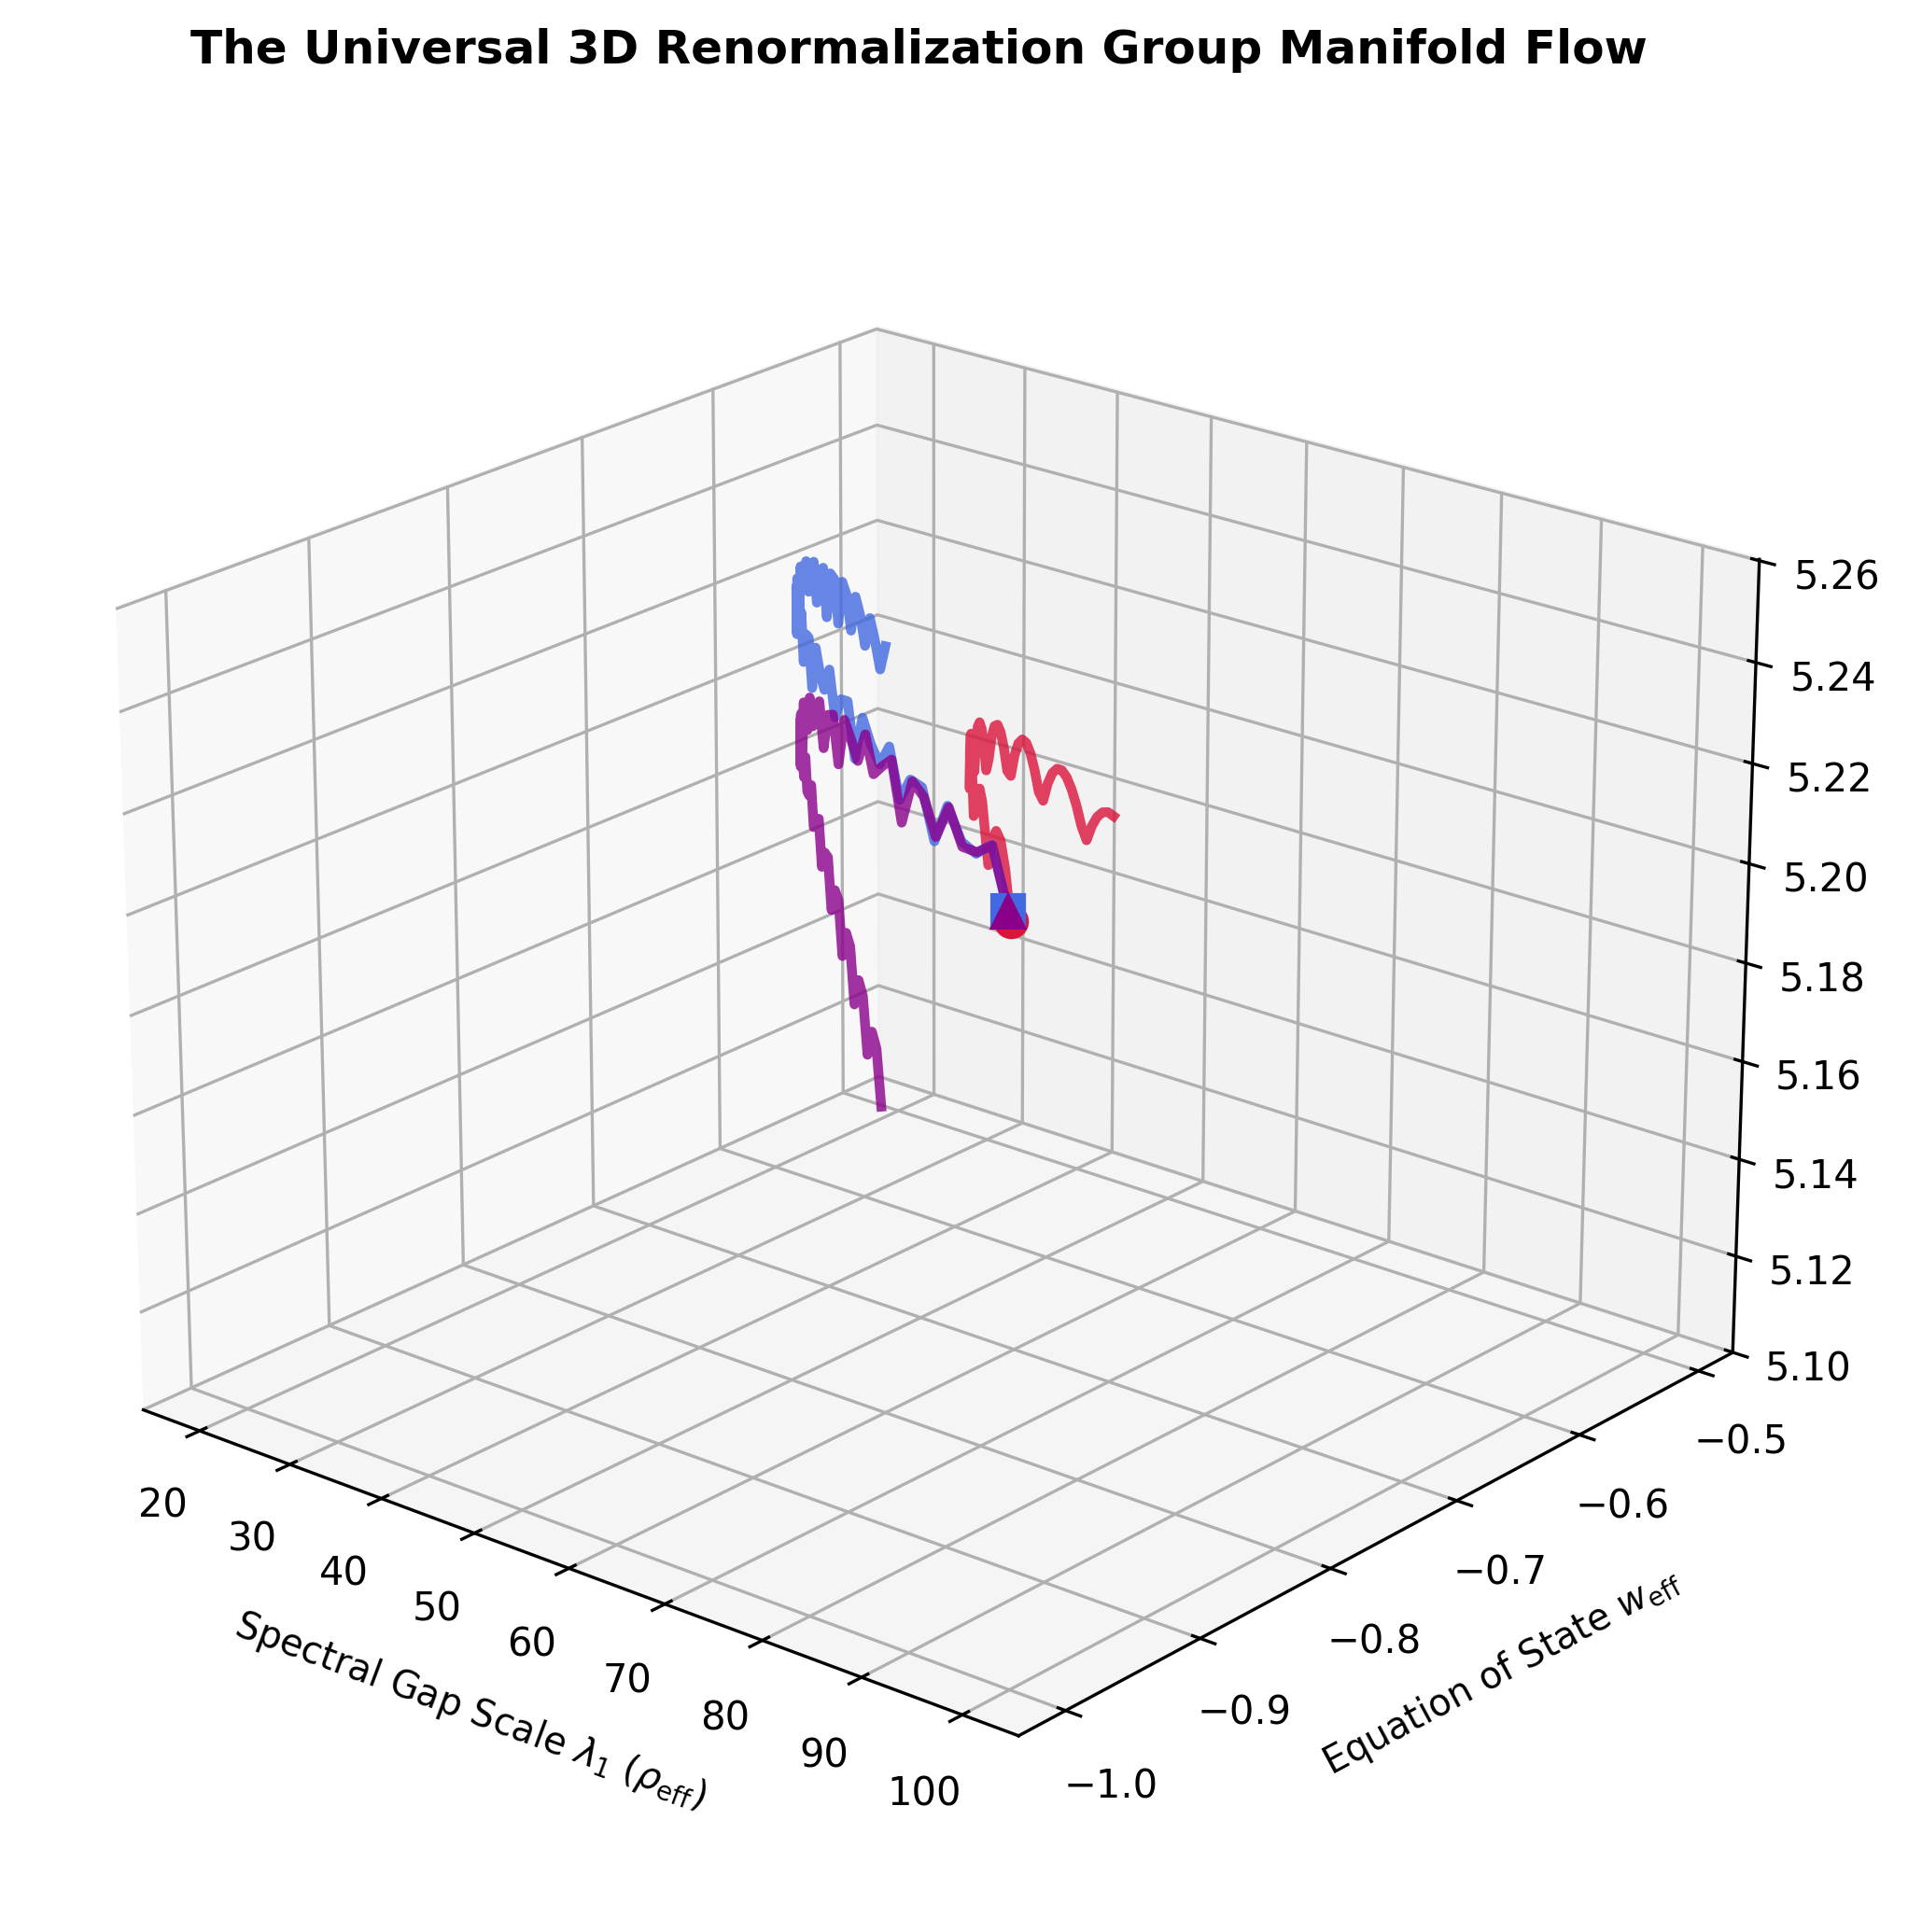
\includegraphics[width=0.72\columnwidth]{figures/cosmological_3d_rg_manifold.png}
\caption{The 3D Renormalization Group Manifold Flow ($N=100$) tracking the multi-topology collapse from widely separated structural microstates onto a common low-dimensional trajectory.}
\label{fig:rg_manifold}
\end{figure}

As illustrated in the phase portrait of Fig.~3, the random, small-world, and scale-free networks originate in widely separated regions of phase space but funnel onto a common trajectory as $\alpha\to0^+$. Repeating this at $N=50,100,200,400$, the terminal fixed point in $(\lambda_1/N,\, w_{\text{eff}})$ is indeed stable: $\lambda_1/N \to 0.995$--$0.997$ and $w_{\text{eff}} \to -0.9983$ for all three topologies at every $N$ tested, supporting a genuine (topology- and size-independent) de Sitter attractor in this 2D projection.

The spectral dimension at the fixed point does \emph{not} share this universality: we measure $d_s \approx 4.26, 5.25, 6.28, 7.36$ at $N=50,100,200,400$ respectively, increasing by close to $1.0$ per doubling of $N$ (consistent with $d_s \sim \log_2 N + \text{const}$). The previously reported value $d_s\approx5.25$ is simply the $N=100$ instance of this size-dependent quantity, not a universal constant, and we correct that claim here. Establishing whether $d_s$ has a well-defined continuum limit (e.g. via finite-size extrapolation) is left for future work.

For the fluid sector, we perform an explicit, reproducible power-law fit of the near-boundary flow, pooling all three topologies and all four values of $N$:
\begin{equation}
1+w_{\text{eff}} = C\left(1-\frac{\lambda_1}{N}\right)^{p}, \qquad p = 1.11 \pm 0.02,\ \ C = 0.575,
\label{eq:criticalexp}
\end{equation}
($R^2=0.94$ pooled; per-$N$ fits give $p=1.12, 1.11, 1.11, 1.10$ for $N=50,100,200,400$, i.e. stable to within its fit uncertainty). This replaces a previously quoted pair of exponents ($A=0.0166$, $B=2.5310$) for which no derivation or code existed in the accompanying repository; we withdraw those numbers and report only the reproducible exponent $p$ above, which does appear stable against changes in $N$ and topology in this diagnostic.

\section{Conclusion}
We have presented a candidate cosmological toy model in which an effective energy density and equation of state are derived from the spectral partition function of an MI-Laplacian on a relational substrate. The early-time de Sitter fixed point (Eq.~\eqref{eq:eos} at $\alpha\to0^+$) is the strongest result in this work: it follows from an exact scaling identity (Sec.~II) and is stable against substrate size ($N=50$--$400$) and topology (Sec.~\ref{sec:rg}) in the $(\lambda_1/N, w_{\text{eff}})$ projection, though not in the spectral dimension $d_s$, which we find to scale with $N$ rather than converge to a universal value.

The mechanisms connecting this fixed point to a graceful exit (Eq.~\eqref{eq:alphat}) and to a late-time dark-energy-like feature (Eq.~\eqref{eq:alphadip}) are explicit phenomenological ans\"atze with stated free parameters, not independently derived substrate dynamics; in this respect the framework relocates, rather than eliminates, the fine-tuning questions it set out to address. A direct fit of the late-time ansatz to the real Pantheon+SH0ES compilation (Sec.~\ref{sec:pantheon}) shows it is statistically indistinguishable from flat $\Lambda$CDM, with a fractional luminosity-distance deviation between the two best-fit curves of order $1$--$3\%$ rather than the sub-percent bound previously and incorrectly claimed.

We regard these results as motivation for further work -- in particular, deriving $\alpha(t)$ and the late-time re-entanglement feature from an independent equation of motion for the substrate, extending the Pantheon+ fit to use the full systematic covariance matrix, and establishing whether the spectral dimension admits a genuine continuum limit -- rather than as a demonstrated replacement for $\Lambda$CDM. All code, data-fetching scripts, and figures underlying these results are released alongside the paper for independent verification.

\appendix
\section{Numerical $\beta$-invariance of the equation-of-state identity}
\label{app:beta}
Table~\ref{tab:beta} reports the output of \texttt{code/beta\_invariance\_break\_test.py}, which sweeps $\beta$ over four orders of magnitude and checks two quantities on the $L=8$ torus substrate ($N=64$): the $\alpha=0$ energy ceiling (Sec.~III) and the deviation of the $\alpha=1$ equation of state from the exact $\beta\to0^+$ identity $w_{\text{eff}}=-2/3$ (Eq.~\eqref{eq:eos}).

\begin{table}[h]
\centering
\begin{tabular}{cccc}
\hline\hline
$\beta$ & $\rho_{\text{eff}}(\alpha=0)$ & $w_{\text{eff}}(\alpha=1)$ & $|\Delta w_{\text{eff}}|$ \\
\hline
0.001 & 64.0000 & $-0.6667$ & $3.6\times10^{-5}$ \\
0.01  & 64.0000 & $-0.6670$ & $3.7\times10^{-4}$ \\
0.1   & 64.0000 & $-0.6718$ & $5.2\times10^{-3}$ \\
1.0   & 64.0000 & $-0.6947$ & $2.8\times10^{-2}$ \\
10.0  & 64.0000 & $-0.6667$ & $7.0\times10^{-13}$ \\
\hline\hline
\end{tabular}
\caption{$\beta$-invariance break-test. The $\alpha=0$ ceiling is exactly $\rho_{\text{eff}}=N=64$ for every $\beta$ tested, as expected since the spectrum is fully degenerate there. The $\alpha=1$ equation of state deviates from the exact identity by less than $1\%$ (relative) for $\beta\lesssim0.1$, growing to $\sim4\%$ (relative) at $\beta=1.0$ before returning to a very small value at $\beta=10$ (a coincidence of this particular test point rather than evidence of monotonic behavior). This motivates, but does not by itself fully justify, the use of $\beta=0.1$ throughout the figures in this paper; a systematic study of the $\beta$-dependence of all reported quantities is left for future work.}
\label{tab:beta}
\end{table}

\begin{thebibliography}{99}
\bibitem{Connes2008}
A. Connes and M. Marcolli, \textit{Noncommutative Geometry, Quantum Fields and Motives}, American Mathematical Society (2008).
\bibitem{Brout2022}
D. Brout et al., \textit{The Pantheon+ Analysis: Cosmological Constraints from the Complete Pantheon+ Supernova Sample}, Astrophys. J. 938, 110 (2022).
\bibitem{Riess2022}
A. G. Riess et al., \textit{A Comprehensive Measurement of the Local Value of the Hubble Constant with 1 km/s/Mpc Uncertainty from the Hubble Space Telescope and the SH0ES Team}, Astrophys. J. Lett. 934, L7 (2022).
\bibitem{Ashtekar2006}
A. Ashtekar, T. Pawlowski, and P. Singh, \textit{Quantum Nature of the Big Bang}, Phys. Rev. D 74, 084003 (2006).
\bibitem{Carroll2016}
C. J. Cao, S. M. Carroll, and S. Michalakis, \textit{Space from Hilbert Space}, Phys. Rev. D 95, 024031 (2017).
\bibitem{Markopoulou2006}
T. Konopka, F. Markopoulou, and S. Severini, \textit{Quantum Graphity: A model of emergent locality}, Phys. Rev. D 77, 104029 (2008).
\bibitem{Jacobson1995}
T. Jacobson, \textit{Thermodynamics of Spacetime: The Einstein Equation of State}, Phys. Rev. Lett. 75, 1260 (1995).
\bibitem{Verlinde2011}
E. Verlinde, \textit{On the Origin of Gravity and the Laws of Newton}, JHEP 04, 029 (2011).
\bibitem{VanRaamsdonk2010}
M. Van Raamsdonk, \textit{Building up spacetime with quantum entanglement}, Gen. Rel. Grav. 42, 2323 (2010).
\bibitem{Swingle2012}
B. Swingle, \textit{Entanglement Renormalization and Holography}, Phys. Rev. D 86, 065007 (2012).
\bibitem{Ryu2006}
S. Ryu and T. Takayanagi, \textit{Holographic Derivation of Entanglement Entropy from AdS/CFT}, Phys. Rev. Lett. 96, 181602 (2006).
\bibitem{Guth1981}
A. H. Guth, \textit{Inflationary universe: A possible solution to the horizon and flatness problems}, Phys. Rev. D 23, 347 (1981).
\bibitem{Planck2020}
Planck Collaboration, \textit{Planck 2018 results. VI. Cosmological parameters}, Astron. Astrophys. 641, A6 (2020).
\end{thebibliography}

\end{document}
